\section{Statistiques descriptives}
\label{sec:stats}

Cette section mesure la pauvreté multidimensionnelle des enfants sénégalais
aux deux vagues et confronte les enfants des ménages bénéficiaires de
transferts à ceux des ménages non bénéficiaires, dimension par dimension et
groupe d'âge par groupe d'âge. L'unité d'observation est l'enfant, et le champ
est celui de l'estimation d'impact~: les 14\,633 enfants suivis
individuellement d'une vague à l'autre et retenus par la définition du
traitement (bénéficiaires en 2018 seulement et jamais bénéficiaires). Les mêmes enfants sont donc décrits en
2018-2019 et en 2021-2022, ce qui rend les tableaux directement comparables
aux coefficients de la section~\ref{sec:resultats}. Toutes les moyennes sont
pondérées par les poids de sondage de l'EHCVM.

Ce choix de champ a une contrepartie qu'il faut avoir en tête à la lecture~:
les enfants vieillissent de trois ans entre les deux passages. Les groupes
d'âge sont donc figés à la période de base - \og 0-4 ans \fg{} se lit \og âgé
de 0 à 4 ans en 2018 \fg{} -, sans quoi une sous-section comparerait des
enfants à d'autres enfants. Il s'ensuit que certaines privations deviennent
applicables en cours de panel~: les enfants de 0 à 4 ans en 2018 en ont 3 à 7
en 2021 et une partie d'entre eux entre dans le champ de l'indicateur de
scolarisation, nul par construction à la première vague.

\subsection{Profil des enfants selon le statut de bénéficiaire du ménage}
\label{subsec:selection}

Le statut de bénéficiaire n'est pas distribué au hasard, et c'est de là que
naît le problème d'identification~: le tableau~\ref{tab:selection} compare les
enfants selon le statut de leur ménage à la période de base.

\begin{table}[H]
  \centering
  \caption[Caractéristiques des enfants selon le statut de transferts du ménage (EHCVM I)]{Caractéristiques des enfants selon le statut de transferts du ménage (EHCVM I)\protect\footnotemark}
  \label{tab:selection}
  \zebre
  \begin{tabular}{|l|c|c|c|}
    \hline
\entete Variable & Bénéficiaires ($D=1$) & Non-bénéf. ($D=0$) & $p$-valeur \\
    \hline
    Caractéristiques de l'enfant & & & \\ \hline
    \quad Filles (\%)             & 49,0  & 49,0  & n.s. \\ \hline
    \quad Âge (années)            & 6,9   & 6,7   & 0,097 \\ \hline
    Caractéristiques du ménage & & & \\ \hline
    \quad Taille du ménage        & 14,28 & 12,49 & 0,035 \\ \hline
    \quad Âge du chef (ans)       & 52,2  & 52,0  & 0,087 \\ \hline
    \quad Chef de ménage féminin (\%) & 31 & 18 & $<$0,001 \\ \hline
    \quad Milieu urbain (\%)      & 53  & 38  & 0,001 \\ \hline
    \quad Dépense par tête (FCFA) & 472~614 & 416~116 & 0,002 \\
    \hline
    Taille d'échantillon ($n$ enfants) & 1~156 & 13~477 & - \\
    \hline
  \end{tabular}

  {\footnotesize \textit{Source :} Calcul de l'auteur, EHCVM.}
\end{table}
\footnotetext{\textit{Note :} enfants de 0 à 17 ans suivis aux deux vagues, mesurés à la période de base, moyennes pondérées par \texttt{hhweight}~; écarts-types clusterisés par grappe. \og n.s. \fg{} : écart non significatif au seuil de 10\,\%.}

La sélection opère sur le ménage, pas sur l'enfant. Les enfants de ménages
bénéficiaires vivent dans des ménages plus grands, plus aisés, plus urbains et
plus souvent dirigés par une femme~; ils ne s'en distinguent en revanche pas
par le sexe, et à peine par l'âge. Une comparaison naïve des trajectoires de pauvreté entre les deux
groupes confondrait donc l'effet des transferts avec ces différences
initiales~: c'est l'objet de l'hypothèse H3, et la raison d'être de la
stratégie exposée au chapitre~\ref{sec:methodo}.

\subsection{Motifs et montants des transferts reçus}

Au-delà du statut binaire de bénéficiaire, le module transferts de l'EHCVM
renseigne, pour chaque transfert reçu, le motif principal déclaré par le
ménage ainsi que le montant et la fréquence des envois. Le
tableau~\ref{tab:motifs_transferts} présente la répartition des motifs pour
les transferts en provenance de l'étranger, en distinguant les motifs
rattachables aux dimensions du bien-être de l'enfant (consommation courante,
santé, éducation, logement)~; les autres motifs déclarés (fêtes et
évènements, appui à une entreprise ou aux champs, achat de terrain) sont
regroupés dans une catégorie résiduelle.

\begin{table}[H]
  \centering
  \caption{Répartition des motifs déclarés des transferts de migrants (\%)}
  \label{tab:motifs_transferts}
  \zebre
  \begin{tabular}{|l|c|c|}
    \hline
\entete Motif principal déclaré & EHCVM I (2018) & EHCVM II (2021) \\
    \hline
    Soutien courant                        & 66,7 & 68,5 \\ \hline
    Santé, maladie                         & 4,6  & 6,5  \\ \hline
    Scolarité, éducation                   & 3,5  & 3,7  \\ \hline
    Construction d'une maison              & 0,7  & 0,7  \\ \hline
    Autres motifs                          & 24,5 & 20,7 \\
    \hline
    Nombre de transferts étrangers         & 2~406 & 2~775 \\
    \hline
  \end{tabular}

  {\footnotesize \textit{Source :} Calcul de l'auteur, EHCVM.}
\end{table}

La structure des motifs est stable entre les deux vagues~:
environ deux transferts sur trois relèvent du soutien courant, c'est-à-dire
d'un appui non affecté au budget général du ménage. Les motifs directement
fléchés vers le capital humain des enfants (scolarité et santé) ne
représentent qu'environ 8 à 10\,\% des transferts déclarés. Cette
prédominance du soutien non affecté conforte le choix de mesurer l'effet des
transferts sur les conditions de vie effectives des enfants (privations
MODA) plutôt que de raisonner sur l'affectation déclarée des fonds~:
l'argent étant fongible au sein du budget du ménage, un transfert de
soutien courant peut financer la scolarité ou les soins, et réciproquement.

\begin{table}[H]
  \centering
  \caption[Montant annuel des transferts étrangers reçus par ménage bénéficiaire (FCFA)]{Montant annuel des transferts étrangers reçus par ménage bénéficiaire (FCFA)\protect\footnotemark}
  \label{tab:montants_transferts}
  \zebre
  \begin{tabular}{|l|c|c|}
    \hline
\entete Statistique & EHCVM I (2018) & EHCVM II (2021) \\
    \hline
    Moyenne              & 883~180   & 948~113   \\ \hline
    Médiane              & 300~000   & 275~000   \\ \hline
    Premier quartile     & 60~000    & 70~000    \\ \hline
    Troisième quartile   & 1~200~000 & 1~200~000 \\
    \hline
    Ménages bénéficiaires ($n$) & 1~584 & 1~765 \\
    \hline
  \end{tabular}

  {\footnotesize \textit{Source :} Calcul de l'auteur, EHCVM.}
\end{table}
\footnotetext{\textit{Note :} montants annualisés, sommés au niveau du ménage.}

Les montants en jeu sont substantiels mais dispersés~: la médiane
s'établit autour de 300~000 FCFA par an (soit un ordre de grandeur comparable
au seuil de pauvreté monétaire par tête), tandis que la moyenne, proche de
900~000 FCFA, est tirée vers le haut par une minorité de gros receveurs (le
troisième quartile atteint 1~200~000 FCFA dans les deux vagues). Rapportée à
la dépense annuelle par tête moyenne des ménages,
cette manne représente une ressource loin d'être marginale pour les ménages
bénéficiaires, ce qui rend d'autant plus plausible un effet mesurable, dans un
sens ou dans l'autre, sur les conditions de vie des enfants.

\subsection{Ensemble 0 à 17 ans}
\label{subsec:ensemble}

En 2018-2019, l'incidence de la pauvreté multidimensionnelle de ces enfants
atteint 65,8\,\%, avec une intensité moyenne $A = 71{,}2\,\%$, soit la part des
sept dimensions en privation parmi les enfants pauvres, et un indice ajusté
$M_0 = 0{,}468$. Cette intensité élevée signifie que les enfants
multidimensionnellement pauvres cumulent en moyenne près de cinq privations sur
sept, bien au-delà du seuil $k=4$. En 2021-2022, l'incidence recule à 59,9\,\%
($A = 70{,}6\,\%$, $M_0 = 0{,}422$), soit une baisse de 5,9 points de
pourcentage de l'incidence et de 0,046 point de l'indice ajusté~: les enfants
sont moins nombreux à être multidimensionnellement pauvres, et ceux qui le
restent cumulent à peine moins de privations simultanées.
La décomposition par milieu montre que la baisse est un peu plus marquée en
milieu urbain (-$7{,}0$ pp~: de 37,5\,\% à 30,5\,\%) qu'en milieu rural
(-$5{,}3$ pp~: de 84,1\,\% à 78,8\,\%), de sorte que l'écart urbain-rural,
déjà considérable en 2018 (46,6 pp), se creuse légèrement (48,3 pp en 2021).

Le c\oe{}ur descriptif de cette sous-section est la comparaison entre les
enfants des ménages bénéficiaires de transferts de migrants et ceux des
ménages non bénéficiaires, aux deux vagues. C'est l'écart entre ces deux groupes,
et surtout la façon dont cet écart évolue entre 2018-2019 et 2021-2022, qui
porte l'information sur l'impact des transferts~: la double différence descriptive
reportée dans la dernière colonne du tableau~\ref{tab:comparaison_benef}
préfigure, sans correction de sélection, l'estimateur PSM-DD de la
section~\ref{sec:resultats}.

\begin{table}[H]
  \centering
  \caption{Taux de privation par dimension selon le statut de bénéficiaire, ensemble des enfants (\%)}
  \label{tab:comparaison_benef}
  \zebre
  \small
  \resizebox{\linewidth}{!}{%
  \begin{tabular}{|l|c|c|c|c|c|c|c|}
    \hline
\entete & \multicolumn{3}{|c|}{EHCVM I (2018-19)} & \multicolumn{3}{|c|}{EHCVM II (2021-22)} & \\ \hline
\entete Dimension & Non-bénéf. & Bénéf. & Écart & Non-bénéf. & Bénéf. & Écart & DD \\
    \hline
    Assainissement         & 55,3 & 38,4 & -16,9$^{***}$ & 52,7 & 37,5 & -15,1$^{***}$ & 1,8 \\ \hline
    Eau                    & 23,7 & 18,3 & -5,3          & 18,3 & 15,1 & -3,1          & 2,2 \\ \hline
    Logement               & 67,6 & 52,9 & -14,6$^{***}$ & 56,7 & 41,6 & -15,2$^{***}$ & -0,5 \\ \hline
    Nutrition              & 73,4 & 58,5 & -14,9$^{***}$ & 66,5 & 59,5 & -7,0$^{**}$   & 7,9 \\ \hline
    Santé                  & 97,4 & 92,1 & -5,4          & 96,3 & 99,1 & 2,8$^{***}$   & 8,2 \\ \hline
    Protection de l'enfant & 65,1 & 67,9 & 2,7           & 64,9 & 66,0 & 1,0$^{*}$     & -1,7 \\ \hline
    Éducation              & 29,2 & 23,6 & -5,7$^{***}$  & 37,0 & 30,8 & -6,2$^{**}$   & -0,5 \\
    \hline
    \hline
    Incidence MODA ($H$) & 67,2 & 49,7 & -17,5$^{***}$ & 61,1 & 45,9 & -15,1$^{***}$ & 2,4 \\
    \hline
  \end{tabular}%
  }

  {\footnotesize \textit{Source :} Calcul de l'auteur, EHCVM. $^{*}p<0{,}10$, $^{**}p<0{,}05$, $^{***}p<0{,}01$.}
\end{table}

Trois enseignements se dégagent. Premièrement, les enfants des ménages
bénéficiaires sont moins privés que les autres, et ce à chaque vague~: 49,7\,\%
contre 67,2\,\% en 2018-2019, 45,9\,\% contre 61,1\,\% en 2021-2022, soit un
avantage de 18 puis 15 points de pourcentage, très significatif. L'avantage se
lit sur six dimensions sur sept, avec des
écarts allant jusqu'à 17 points en assainissement et 15 en nutrition.
Cet écart de niveau ne mesure toutefois pas un effet des transferts~: il
reflète en grande partie la sélection positive des ménages bénéficiaires,
initialement plus aisés et plus urbains (tableau~\ref{tab:selection}), que
corrige l'appariement. Deuxièmement, la protection de l'enfant fait exception
et s'inverse~: les
enfants des ménages bénéficiaires y sont un peu plus privés que les autres.
Ce résultat est mécanique autant
que substantiel~: cette dimension inclut le fait de ne pas vivre avec ses
deux parents biologiques, situation consubstantielle au départ en migration
d'un membre du ménage qui définit précisément le statut de bénéficiaire.
Troisièmement, et c'est le point qui intéresse l'évaluation d'impact, l'écart
entre les deux groupes se resserre légèrement entre les deux vagues. La
double différence descriptive sur l'incidence MODA est de 2,4 points
(l'avantage des bénéficiaires se réduit de 17,5 à 15,1 points), et elle est
portée par deux dimensions, la santé (8,2 points) et la nutrition
(7,9 points). Ce chiffre est du même signe que l'effet estimé de la
section~\ref{sec:resultats}, sans qu'aucune dimension prise isolément n'y
produise de coefficient significatif.

\begin{figure}[H]
  \centering
  \caption{Évolution de l'incidence MODA entre EHCVM I et EHCVM II : enfants des ménages bénéficiaires et non bénéficiaires}
  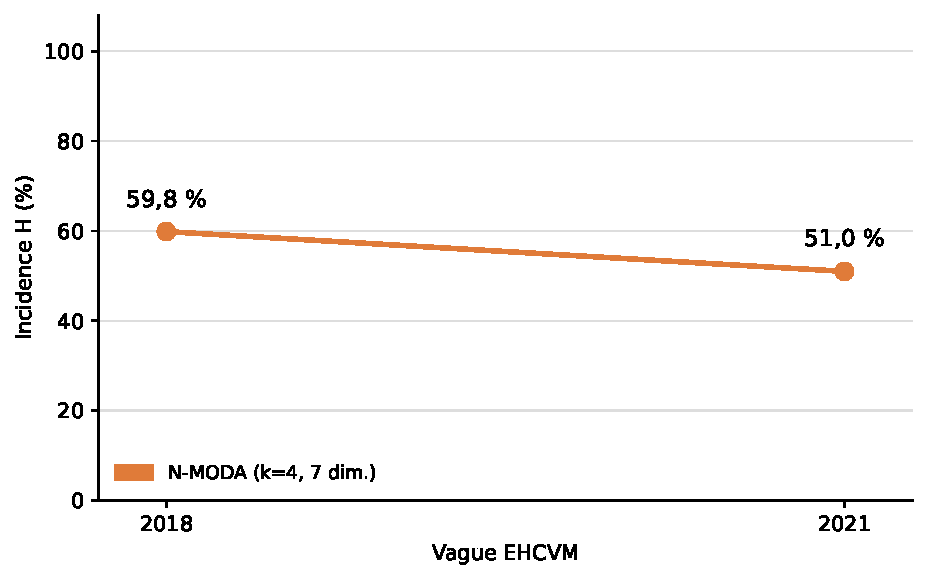
\includegraphics[width=0.85\linewidth]{figures/fig_evolution_ipm.pdf}
  \label{fig:evolution_ipm}

  {\footnotesize \textit{Source :} Calcul de l'auteur, EHCVM.}
\end{figure}

La figure~\ref{fig:evolution_ipm} met en évidence le quasi-parallélisme des
deux trajectoires, qui reculent conjointement, l'écart entre elles se refermant
à peine. Cette comparaison est déclinée groupe d'âge par groupe d'âge dans les
sous-sections~\ref{subsec:age_0_4} à~\ref{subsec:age_15_17}.

Le tableau~\ref{tab:prevalence_dim} décompose les taux de privation par
dimension pour l'ensemble des enfants. La dimension santé (combustible solide
pour cuisiner ou absence d'accès à pied à une structure de santé) est la
privation la plus répandue, touchant environ 97\,\% des enfants aux deux
vagues. Viennent ensuite la nutrition, mesurée par l'échelle FIES (\emph{Food
Insecurity Experience Scale}) de l'insécurité alimentaire vécue, la protection
de l'enfant et le logement inadéquat. Cette dernière dimension est celle qui
s'améliore le plus entre les deux vagues (-$10{,}9$ pp), tandis que l'éducation
progresse de 7,7 points. Cette hausse n'est pas une dégradation~: elle tient
pour l'essentiel au vieillissement du panel, l'indicateur de scolarisation
devenant applicable à des enfants qui étaient trop jeunes en 2018.

\begin{table}[H]
  \centering
  \caption[Taux de privation par dimension MODA (enfants 0-17 ans, \%)]{Taux de privation par dimension MODA (enfants 0-17 ans, \%)\protect\footnotemark}
  \label{tab:prevalence_dim}
  \zebre
  \begin{tabularx}{\linewidth}{|X|c|c|c|}
    \hline
\entete Dimension & EHCVM I & EHCVM II & Variation (pp) \\
    \hline
    Assainissement     & 53,9 & 51,5 & -$2{,}4$ \\ \hline
    Eau                & 23,2 & 18,0 & -$5{,}2$ \\ \hline
    Logement           & 66,4 & 55,5 & -$10{,}9$ \\ \hline
    Nutrition          & 72,2 & 65,9 & -$6{,}3$ \\ \hline
    Santé              & 97,0 & 96,5 & -$0{,}5$ \\ \hline
    Protection de l'enfant & 65,3 & 65,0 & -$0{,}3$ \\ \hline
    Éducation          & 28,8 & 36,5 & $7{,}7$ \\
    \hline
    \hline
    \multicolumn{4}{|c|}{Indice MODA} \\ \hline
    \quad Incidence $H$ (\%)                           & 65,8 & 59,9 & -$5{,}9$ \\ \hline
    \quad Intensité $A$ (\%)                           & 71,2 & 70,6 & -$0{,}6$ \\ \hline
    \quad Indice ajusté $M_0$                          & 0,468 & 0,422 & -$0{,}046$ \\
    \hline
  \end{tabularx}

  {\footnotesize \textit{Source :} Calcul de l'auteur, EHCVM.}
\end{table}
\footnotetext{\textit{Note :} définition détaillée des indicateurs de chaque dimension en annexe~\ref{ann:C}.}

Le tableau~\ref{tab:moda_age} récapitule l'incidence par groupe d'âge de la
période de base. En 2018, les enfants de 5 à 14 ans affichent le taux le plus
élevé (69,8\,\%), du fait des privations éducatives cumulées aux privations de
logement et d'assainissement. Le classement s'inverse en 2021~: cette tranche
enregistre le recul le plus net (-$10{,}7$ pp) et passe sous les deux autres,
tandis que les enfants de 0 à 4 ans en 2018 voient leur incidence augmenter de
2,6 points. Cette hausse est la contrepartie du vieillissement déjà signalé~:
scolarisables en 2021, ces enfants sont désormais évalués sur sept dimensions
au lieu de six, ce qui relève mécaniquement leur probabilité d'atteindre le
seuil de quatre privations.

\begin{table}[H]
  \centering
  \caption{Incidence MODA par groupe d'âge à la période de base : EHCVM I (2018-2019) et EHCVM II (2021-2022)}
  \label{tab:moda_age}
  \zebre
  \begin{tabular}{|l|c|c|}
    \hline
\entete Groupe d'âge en 2018 & \multicolumn{2}{|c|}{$H$ (\%)} \\ \hline

                 & EHCVM I & EHCVM II \\
    \hline
    0-4 ans     & 59,1 & 61,7 \\ \hline
    5-14 ans    & 69,8 & 59,1 \\ \hline
    15-17 ans   & 59,9 & 54,1 \\
    \hline
    Ensemble 0-17 ans & 65,8 & 59,9 \\
    \hline
  \end{tabular}

  {\footnotesize \textit{Source :} Calcul de l'auteur, EHCVM.}
\end{table}

\begin{table}[H]
  \centering
  \caption{Incidence MODA selon le sexe de l'enfant et le statut du ménage, ensemble des enfants (\%)}
  \label{tab:sexe_ensemble}
  \zebre
  \small
  \resizebox{\linewidth}{!}{%
  \begin{tabular}{|l|c|c|c|c|c|c|c|}
    \hline
\entete & \multicolumn{3}{|c|}{EHCVM I (2018-19)} & \multicolumn{3}{|c|}{EHCVM II (2021-22)} & \\ \hline
\entete Sexe de l'enfant & Non-bénéf. & Bénéf. & Écart & Non-bénéf. & Bénéf. & Écart & DD \\
    \hline
    Garçons & 66,0 & 45,7 & -20,3$^{***}$ & 60,4 & 44,9 & -15,5$^{***}$ & 4,8 \\ \hline
    Filles & 68,5 & 53,9 & -14,6$^{***}$ & 61,8 & 47,1 & -14,7$^{***}$ & -0,1 \\
    \hline
  \end{tabular}%
  }

  {\footnotesize \textit{Source :} Calcul de l'auteur, EHCVM. 7\,355 garçons et 7\,278 filles. $^{***}p<0{,}01$.}
\end{table}

Le tableau~\ref{tab:sexe_ensemble} croise le sexe de l'enfant avec le statut
du ménage et la vague, croisement que l'hypothèse H2 appelle directement.
L'avantage des enfants de ménages bénéficiaires existe pour les deux sexes,
mais son évolution diverge~: la double différence descriptive vaut
4,8 points chez les garçons et -0,1 point chez les filles. L'écart de niveau
initial est plus large chez les garçons (20,3 points contre 14,6), et c'est
chez eux seulement qu'il se resserre~; l'estimation d'impact retrouvera ce
contraste sans parvenir à l'établir statistiquement
(section~\ref{sec:discussion}).

\begin{table}[H]
  \centering
  \caption{Incidence MODA selon le quintile de montant reçu, ensemble des enfants (\%)}
  \label{tab:quintile_ensemble}
  \zebre
  \begin{tabular}{|l|r|c|c|c|}
    \hline
\entete Groupe & Médiane reçue & EHCVM I & EHCVM II & DD \\
    \hline
    Non-bénéficiaires & --- & 67,2 & 61,1 & réf. \\ \hline
    Quintile 1 &    29~000 & 68,2 & 69,3 & 7,2   \\ \hline
    Quintile 2 &   110~000 & 61,6 & 61,4 & 5,9   \\ \hline
    Quintile 3 &   325~000 & 56,3 & 51,6 & 1,5   \\ \hline
    Quintile 4 &   780~000 & 37,2 & 32,8 & 1,7   \\ \hline
    Quintile 5 & 2~070~000 & 31,1 & 21,4 & -3,6  \\
    \hline
  \end{tabular}

  {\footnotesize \textit{Source :} Calcul de l'auteur, EHCVM. Montants en FCFA par an.}
\end{table}

Le tableau~\ref{tab:quintile_ensemble} découpe les ménages bénéficiaires
selon le montant annuel reçu, ce que le volet intensité de l'hypothèse H2
appelle. Deux régularités s'en dégagent. L'incidence décroît fortement avec le
montant à chaque vague~: du premier au cinquième quintile, elle passe de
68,2\,\% à 31,1\,\% en 2018 et de 69,3\,\% à 21,4\,\% en 2021. Et le décrochage
relatif aux non-bénéficiaires se concentre sur le bas de la distribution~: la
double différence vaut 7,2 puis 5,9 points dans les deux premiers quintiles,
s'atténue au milieu et devient négative dans le dernier. Les enfants des
ménages recevant les montants les plus faibles sont donc à la fois les plus
privés et ceux dont la situation se dégrade le plus, relativement aux
non-bénéficiaires~; l'estimation retrouvera ce profil décroissant sans
parvenir à l'établir (section~\ref{sec:discussion}).

\subsection{Enfants de 0 à 4 ans}
\label{subsec:age_0_4}

Cette tranche réunit 5\,089 enfants âgés de 0 à 4 ans en 2018-2019, qui en ont
3 à 7 en 2021-2022. Son incidence MODA passe de 59,1\,\% à 61,7\,\%, seule
progression des trois groupes. Cette hausse ne traduit pas une dégradation des
conditions de vie mais l'élargissement du champ de mesure~: l'éducation,
inapplicable à cet âge en 2018, concerne 43,8\,\% d'entre eux en 2021, quand
les six autres dimensions reculent ou stagnent (tableau~\ref{tab:dim_0_4}).

\begin{table}[H]
  \centering
  \caption{Taux de privation par dimension, enfants de 0 à 4 ans (\%)}
  \label{tab:dim_0_4}
  \zebre
  \begin{tabularx}{\linewidth}{|X|c|c|c|}
    \hline
\entete Dimension & EHCVM I & EHCVM II & Variation (pp) \\
    \hline
    Assainissement     & 55,2 & 52,5 & -$2{,}7$ \\ \hline
    Eau                & 25,0 & 19,3 & -$5{,}7$ \\ \hline
    Logement           & 67,6 & 57,9 & -$9{,}7$ \\ \hline
    Nutrition          & 72,2 & 66,2 & -$6{,}0$ \\ \hline
    Santé              & 96,6 & 96,9 & $0{,}3$ \\ \hline
    Protection de l'enfant & 53,1 & 58,4 & $5{,}3$ \\ \hline
    Éducation          & Non applicable & 43,8 & --- \\
    \hline
    \hline
    Incidence MODA ($H$) & 59,1 & 61,7 & $2{,}6$ \\
    \hline
  \end{tabularx}

  {\footnotesize \textit{Source :} Calcul de l'auteur, EHCVM.}
\end{table}

Le profil de privations des tout-petits se distingue sur deux points. La
protection est la moins fréquente des trois tranches en 2018 (53,1\,\% contre
73,0\,\% chez les 5-14 ans), l'indicateur ne combinant à cet âge que
l'absence d'acte de naissance et la séparation parentale, sans le volet
travail des enfants~; elle progresse ensuite de 5,3 points, à mesure que ces
enfants entrent dans le champ de l'indicateur complet. À l'inverse, l'eau et
le logement les touchent davantage que les aînés, ces privations étant
mesurées au niveau du logement et les jeunes enfants vivant dans les ménages
les plus nombreux. La nutrition touche
ici plus de six enfants sur dix aux deux vagues.

\begin{table}[H]
  \centering
  \caption[Taux de privation selon le statut de bénéficiaire, enfants de 0 à 4 ans (\%)]{Taux de privation par dimension selon le statut de bénéficiaire, enfants de 0 à 4 ans (\%)\protect\footnotemark}
  \label{tab:statut_0_4}
  \zebre
  \small
  \resizebox{\linewidth}{!}{%
  \begin{tabular}{|l|c|c|c|c|c|c|c|}
    \hline
\entete & \multicolumn{3}{|c|}{EHCVM I (2018-19)} & \multicolumn{3}{|c|}{EHCVM II (2021-22)} & \\ \hline
\entete Dimension & Non-bénéf. & Bénéf. & Écart & Non-bénéf. & Bénéf. & Écart & DD \\
    \hline
    Assainissement & 56,7 & 36,9 & -19,9$^{***}$ & 54,0 & 33,8 & -20,3$^{***}$ & -0,4 \\ \hline
    Eau & 25,5 & 19,2 & -6,3 & 19,6 & 15,5 & -4,1 & 2,2 \\ \hline
    Logement & 69,1 & 50,0 & -19,1$^{***}$ & 59,2 & 41,8 & -17,4$^{**}$ & 1,7 \\ \hline
    Nutrition & 73,8 & 53,4 & -20,4$^{***}$ & 67,0 & 57,3 & -9,6$^{**}$ & 10,8 \\ \hline
    Santé & 97,1 & 90,7 & -6,4 & 96,7 & 99,1 & 2,4$^{***}$ & 8,8 \\ \hline
    Protection de l'enfant & 53,1 & 54,3 & 1,2 & 58,2 & 60,6 & 2,4$^{*}$ & 1,1 \\ \hline
    Éducation & \multicolumn{3}{|c|}{Non applicable} & 44,1 & 39,1 & -5,0 & --- \\
    \hline
    Incidence MODA ($H$) & 60,7 & 39,6 & -21,1$^{***}$ & 62,9 & 47,6 & -15,2$^{***}$ & 5,9 \\
    \hline
  \end{tabular}%
  }

  {\footnotesize \textit{Source :} Calcul de l'auteur, EHCVM.}
\end{table}
\footnotetext{\textit{Note :} 5\,089 enfants observés aux deux vagues, pondéré par \texttt{hhweight}. \og Écart \fg{} = bénéficiaires moins non-bénéficiaires~; \og DD \fg{} = évolution de cet écart. Significativité de l'écart testée par régression avec erreurs-types clusterisées par grappe~: $^{*}p<0{,}10$, $^{**}p<0{,}05$, $^{***}p<0{,}01$.}

La comparaison selon le statut de bénéficiaire
(tableau~\ref{tab:statut_0_4}) est celle qui intéresse l'évaluation d'impact.
Les tout-petits des ménages bénéficiaires sont nettement moins souvent pauvres
que les autres, 39,6\,\% contre 60,7\,\% en 2018 et 47,6\,\% contre
62,9\,\% en 2021, et l'avantage se lit sur cinq dimensions sur six en 2018. Il
est le plus large en nutrition (20,4 points) et en assainissement
(19,9 points). La protection fait exception et s'inverse~: les tout-petits des
ménages bénéficiaires y sont un peu plus privés, l'absence
d'un parent parti en migration alimentant directement l'indicateur.

C'est surtout l'évolution de cet écart qui retient l'attention. L'avantage des
bénéficiaires se réduit de 21,1 à 15,2 points, soit une double différence
descriptive de 5,9 points, la plus forte des trois tranches. Elle est portée
avant tout par la nutrition, dont l'écart passe de 20,4 à 9,6 points, soit
10,8 points de resserrement à elle seule, et par la santé (8,8 points).
L'estimation d'impact ne produira toutefois de coefficient significatif ni
sur cette tranche ni sur ces dimensions (section~\ref{sec:discussion})~: le
constat descriptif suggère plus qu'il n'établit.

\begin{table}[H]
  \centering
  \caption{Incidence MODA selon le sexe de l'enfant et le statut du ménage, enfants de 0 à 4 ans (\%)}
  \label{tab:sexe_0_4}
  \zebre
  \small
  \resizebox{\linewidth}{!}{%
  \begin{tabular}{|l|c|c|c|c|c|c|c|}
    \hline
\entete & \multicolumn{3}{|c|}{EHCVM I (2018-19)} & \multicolumn{3}{|c|}{EHCVM II (2021-22)} & \\ \hline
\entete Sexe de l'enfant & Non-bénéf. & Bénéf. & Écart & Non-bénéf. & Bénéf. & Écart & DD \\
    \hline
    Garçons & 60,1 & 37,3 & -22,8$^{***}$ & 62,6 & 46,5 & -16,1$^{**}$ & 6,7 \\ \hline
    Filles & 61,3 & 42,3 & -19,0$^{***}$ & 63,2 & 49,0 & -14,2$^{**}$ & 4,8 \\
    \hline
  \end{tabular}%
  }

  {\footnotesize \textit{Source :} Calcul de l'auteur, EHCVM. 2\,606 garçons et 2\,483 filles. $^{**}p<0{,}05$, $^{***}p<0{,}01$.}
\end{table}

La lecture par sexe (tableau~\ref{tab:sexe_0_4}) montre que le resserrement
touche les deux sexes, un peu plus les garçons, dont la double différence
descriptive atteint 6,7 points contre 4,8 chez les filles. Les garçons
partaient de l'incidence la plus basse de la tranche (37,3\,\% en 2018, soit
22,8 points sous leurs homologues de ménages non bénéficiaires) et perdent
un quart de cet avantage en trois ans.

\begin{table}[H]
  \centering
  \caption{Incidence MODA selon le quintile de montant reçu, enfants de 0 à 4 ans (\%)}
  \label{tab:quintile_0_4}
  \zebre
  \begin{tabular}{|l|r|c|c|c|}
    \hline
\entete Groupe & Médiane reçue & EHCVM I & EHCVM II & DD \\
    \hline
    Non-bénéficiaires & --- & 60,7 & 62,9 & réf. \\ \hline
    Quintile 1 &    29~000 & 56,4 & 82,0 & 23,5 \\ \hline
    Quintile 2 &   110~000 & 55,1 & 60,2 & 2,9  \\ \hline
    Quintile 3 &   325~000 & 43,7 & 45,8 & -0,1 \\ \hline
    Quintile 4 &   780~000 & 25,9 & 37,4 & 9,4  \\ \hline
    Quintile 5 & 2~070~000 & 26,7 & 24,4 & -4,5 \\
    \hline
  \end{tabular}

  {\footnotesize \textit{Source :} Calcul de l'auteur, EHCVM. Montants en FCFA par an.}
\end{table}

Chez les tout-petits, le profil du tableau~\ref{tab:quintile_0_4} suit celui
de l'ensemble mais avec un premier quintile nettement détaché~: la double
différence y atteint 23,5 points, contre -4,5 points dans le dernier. Les
effectifs par case sont toutefois réduits, entre 63 et 97 enfants, ce qui
invite à lire le sens du profil plutôt que la valeur de chaque ligne.

\subsection{Enfants de 5 à 14 ans}
\label{subsec:age_5_14}

Les 5-14 ans forment le groupe le plus nombreux, avec 9\,166 enfants, et le
plus exposé en 2018 : leur incidence MODA atteint 69,8\,\%, plus de dix points
au-dessus des 0-4 ans. C'est aussi le groupe dont la situation s'améliore le
plus nettement, l'incidence tombant à 59,1\,\% en 2021, soit un recul de
10,7 points.

\begin{table}[H]
  \centering
  \caption{Taux de privation par dimension, enfants de 5 à 14 ans (\%)}
  \label{tab:dim_5_14}
  \zebre
  \begin{tabularx}{\linewidth}{|X|c|c|c|}
    \hline
\entete Dimension & EHCVM I & EHCVM II & Variation (pp) \\
    \hline
    Assainissement     & 53,4 & 51,1 & -$2{,}3$ \\ \hline
    Eau                & 22,4 & 17,3 & -$5{,}1$ \\ \hline
    Logement           & 65,8 & 54,4 & -$11{,}4$ \\ \hline
    Nutrition          & 72,2 & 65,6 & -$6{,}6$ \\ \hline
    Santé              & 97,1 & 96,2 & -$0{,}9$ \\ \hline
    Protection de l'enfant & 73,0 & 69,1 & -$3{,}9$ \\ \hline
    Éducation          & 44,7 & 32,7 & -$12{,}0$ \\
    \hline
    \hline
    Incidence MODA ($H$) & 69,8 & 59,1 & -$10{,}7$ \\
    \hline
  \end{tabularx}

  {\footnotesize \textit{Source :} Calcul de l'auteur, EHCVM.}
\end{table}

Deux dimensions expliquent la position initiale de cette tranche. La
protection y culmine à 73,0\,\%, l'indicateur combinant à cet âge l'absence
d'acte de naissance, le travail des enfants et la séparation parentale, soit
les trois volets à la fois. L'éducation, mesurée par la non-scolarisation,
touche 44,7\,\% des enfants du groupe, alors qu'elle ne s'applique pas aux
0-4 ans en 2018.

L'éducation explique aussi une bonne part du recul ultérieur~: elle perd
12,0 points, la plus forte baisse de toutes les dimensions et de toutes les
tranches. Une partie de ces enfants a entre-temps dépassé 14 ans et relève
désormais de l'illettrisme et non plus de la scolarisation, indicateur moins
fréquemment en privation. La baisse du logement (-$11{,}4$ pp), elle, est bien
une amélioration des conditions matérielles, commune aux trois tranches.

\begin{table}[H]
  \centering
  \caption[Taux de privation selon le statut de bénéficiaire, enfants de 5 à 14 ans (\%)]{Taux de privation par dimension selon le statut de bénéficiaire, enfants de 5 à 14 ans (\%)\protect\footnotemark}
  \label{tab:statut_5_14}
  \zebre
  \small
  \resizebox{\linewidth}{!}{%
  \begin{tabular}{|l|c|c|c|c|c|c|c|}
    \hline
\entete & \multicolumn{3}{|c|}{EHCVM I (2018-19)} & \multicolumn{3}{|c|}{EHCVM II (2021-22)} & \\ \hline
\entete Dimension & Non-bénéf. & Bénéf. & Écart & Non-bénéf. & Bénéf. & Écart & DD \\
    \hline
    Assainissement & 54,6 & 38,8 & -15,8$^{***}$ & 52,0 & 39,7 & -12,3$^{***}$ & 3,5 \\ \hline
    Eau & 22,8 & 17,7 & -5,2 & 17,5 & 15,1 & -2,4 & 2,8 \\ \hline
    Logement & 66,8 & 53,9 & -12,9$^{***}$ & 55,5 & 41,6 & -14,0$^{**}$ & -1,1 \\ \hline
    Nutrition & 73,2 & 61,8 & -11,4$^{***}$ & 66,1 & 59,5 & -6,5$^{*}$ & 4,9 \\ \hline
    Santé & 97,5 & 92,5 & -5,0$^{*}$ & 95,9 & 99,0 & 3,0$^{***}$ & 8,1 \\ \hline
    Protection de l'enfant & 72,8 & 75,7 & 3,0 & 69,1 & 69,4 & 0,3 & -2,6 \\ \hline
    Éducation & 45,4 & 35,9 & -9,5$^{***}$ & 33,2 & 26,8 & -6,4 & 3,1 \\ \hline
    \hline
    Incidence MODA ($H$) & 71,1 & 54,4 & -16,8$^{***}$ & 60,3 & 45,2 & -15,1$^{***}$ & 1,6 \\
    \hline
  \end{tabular}%
  }

  {\footnotesize \textit{Source :} Calcul de l'auteur, EHCVM.}
\end{table}
\footnotetext{\textit{Note :} 9\,166 enfants observés aux deux vagues, pondéré par \texttt{hhweight}. \og Écart \fg{} = bénéficiaires moins non-bénéficiaires~; \og DD \fg{} = évolution de cet écart. Significativité de l'écart testée par régression avec erreurs-types clusterisées par grappe~: $^{*}p<0{,}10$, $^{**}p<0{,}05$, $^{***}p<0{,}01$.}

Le tableau~\ref{tab:statut_5_14} décline la même comparaison selon le statut
de bénéficiaire. L'avantage des enfants de ménages bénéficiaires est du même
ordre que chez les tout-petits, 54,4\,\% contre 71,1\,\% en 2018 et
45,2\,\% contre 60,3\,\% en 2021, et il se retrouve sur six dimensions sur
sept, protection exceptée. L'éducation le fait apparaître de façon nette~:
35,9\,\% des enfants de ménages bénéficiaires ne sont pas scolarisés, contre
45,4\,\% des autres.

Contrairement aux 0-4 ans, l'écart ne bouge guère entre les deux
vagues~: la double différence descriptive sur l'incidence est de 1,6 point.
Elle reste sensible sur la santé (8,1 points), la nutrition
(4,9 points) et l'assainissement (3,5 points), mais ces mouvements se
compensent en partie avec ceux du logement
(-$1{,}1$ point) et de la protection (-$2{,}6$ points). Les deux groupes
suivent donc des trajectoires quasi
parallèles dans cette tranche, celle qui pèse pourtant le plus lourd dans
l'échantillon.

\begin{table}[H]
  \centering
  \caption{Incidence MODA selon le sexe de l'enfant et le statut du ménage, enfants de 5 à 14 ans (\%)}
  \label{tab:sexe_5_14}
  \zebre
  \small
  \resizebox{\linewidth}{!}{%
  \begin{tabular}{|l|c|c|c|c|c|c|c|}
    \hline
\entete & \multicolumn{3}{|c|}{EHCVM I (2018-19)} & \multicolumn{3}{|c|}{EHCVM II (2021-22)} & \\ \hline
\entete Sexe de l'enfant & Non-bénéf. & Bénéf. & Écart & Non-bénéf. & Bénéf. & Écart & DD \\
    \hline
    Garçons & 69,5 & 50,2 & -19,3$^{***}$ & 59,2 & 44,1 & -15,1$^{**}$ & 4,2 \\ \hline
    Filles & 72,8 & 58,4 & -14,4$^{***}$ & 61,4 & 46,2 & -15,1$^{***}$ & -0,8 \\
    \hline
  \end{tabular}%
  }

  {\footnotesize \textit{Source :} Calcul de l'auteur, EHCVM. 4\,568 garçons et 4\,598 filles. $^{**}p<0{,}05$, $^{***}p<0{,}01$.}
\end{table}

Le croisement par sexe (tableau~\ref{tab:sexe_5_14}) retrouve le contraste
de l'ensemble~: l'écart se resserre chez les garçons (4,2 points) et reste
stable chez les filles (-0,8 point). L'écart de niveau initial est plus
large chez les garçons, et c'est chez eux qu'il se referme.

\begin{table}[H]
  \centering
  \caption{Incidence MODA selon le quintile de montant reçu, enfants de 5 à 14 ans (\%)}
  \label{tab:quintile_5_14}
  \zebre
  \begin{tabular}{|l|r|c|c|c|}
    \hline
\entete Groupe & Médiane reçue & EHCVM I & EHCVM II & DD \\
    \hline
    Non-bénéficiaires & --- & 71,1 & 60,3 & réf. \\ \hline
    Quintile 1 &    29~000 & 73,2 & 64,9 & 2,5   \\ \hline
    Quintile 2 &   110~000 & 64,0 & 62,0 & 8,8   \\ \hline
    Quintile 3 &   325~000 & 62,8 & 54,5 & 2,5   \\ \hline
    Quintile 4 &   780~000 & 42,4 & 29,6 & -2,0  \\ \hline
    Quintile 5 & 2~070~000 & 32,9 & 19,2 & -2,8  \\
    \hline
  \end{tabular}

  {\footnotesize \textit{Source :} Calcul de l'auteur, EHCVM. Montants en FCFA par an.}
\end{table}

Le tableau~\ref{tab:quintile_5_14} montre que la stabilité d'ensemble de cette
tranche recouvre des mouvements contrastés. Les deux premiers quintiles
décrochent, de 2,5 et 8,8 points, tandis que les deux derniers convergent
légèrement vers les non-bénéficiaires~: le profil décroissant selon le
montant se retrouve, atténué, dans cette tranche.

\subsection{Enfants de 15 à 17 ans}
\label{subsec:age_15_17}

Cette tranche ne compte que 378 enfants. Le suivi individuel en est la cause~:
un enfant de 15 à 17 ans en 2018 en a 18 à 20 en 2021 et sort du champ de
l'étude, si bien que seuls subsistent ceux qui avaient tout juste 15 ans à la
première vague. Leur incidence MODA recule de 59,9\,\% à 54,1\,\%.

Cet effectif ne permet pas une analyse comparable à celle des deux autres
tranches. Les résultats sont rapportés pour mémoire, mais les écarts entre
bénéficiaires et non-bénéficiaires n'y sont significatifs sur aucune dimension
à la première vague, et les effectifs par case tombent à quelques dizaines
d'enfants dès que l'on croise le statut avec le sexe ou le montant reçu. C'est
la même limite qui prive l'estimation d'impact de tout coefficient
interprétable sur cette tranche (section~\ref{sec:discussion}).

\begin{table}[H]
  \centering
  \caption[Taux de privation selon le statut de bénéficiaire, enfants de 15 à 17 ans (\%)]{Taux de privation par dimension selon le statut de bénéficiaire, enfants de 15 à 17 ans (\%)\protect\footnotemark}
  \label{tab:statut_15_17}
  \zebre
  \small
  \resizebox{\linewidth}{!}{%
  \begin{tabular}{|l|c|c|c|c|c|c|c|}
    \hline
\entete & \multicolumn{3}{|c|}{EHCVM I (2018-19)} & \multicolumn{3}{|c|}{EHCVM II (2021-22)} & \\ \hline
\entete Dimension & Non-bénéf. & Bénéf. & Écart & Non-bénéf. & Bénéf. & Écart & DD \\
    \hline
    Assainissement & 50,2 & 45,9 & -4,3 & 48,9 & 35,6 & -13,4 & -9,1 \\ \hline
    Eau & 18,4 & 22,9 & 4,5 & 20,5 & 13,3 & -7,2$^{**}$ & -11,7 \\ \hline
    Logement & 65,9 & 65,0 & -1,0 & 51,5 & 39,6 & -11,9$^{*}$ & -10,9 \\ \hline
    Nutrition & 75,4 & 50,6 & -24,8$^{**}$ & 70,1 & 79,7 & 9,5 & 34,3 \\ \hline
    Santé & 99,5 & 97,2 & -2,3 & 98,2 & 100,0 & 1,8 & 4,1 \\ \hline
    Protection de l'enfant & 40,5 & 58,8 & 18,3 & 54,2 & 55,9 & 1,7 & -16,6 \\ \hline
    Éducation & 32,1 & 32,0 & -0,1 & 32,5 & 21,8 & -10,7 & -10,6 \\ \hline
    \hline
    Incidence MODA ($H$) & 59,3 & 64,2 & 4,9 & 55,5 & 43,3 & -12,2 & -17,1 \\
    \hline
  \end{tabular}%
  }

  {\footnotesize \textit{Source :} Calcul de l'auteur, EHCVM.}
\end{table}
\footnotetext{\textit{Note :} 378 enfants observés aux deux vagues, pondéré par \texttt{hhweight}. \og Écart \fg{} = bénéficiaires moins non-bénéficiaires~; \og DD \fg{} = évolution de cet écart. Significativité de l'écart testée par régression avec erreurs-types clusterisées par grappe~: $^{*}p<0{,}10$, $^{**}p<0{,}05$, $^{***}p<0{,}01$.}

Le tableau~\ref{tab:statut_15_17} se distingue de ceux des deux autres
tranches sur un point~: l'avantage de niveau des enfants de ménages
bénéficiaires n'y apparaît pas en 2018, l'incidence y étant même légèrement
supérieure chez les bénéficiaires (64,2\,\% contre 59,3\,\%), sans que l'écart
soit significatif. Seule la nutrition présente un écart net à la première
vague, de 24,8 points. Aucune des évolutions rapportées dans la dernière
colonne ne repose sur des effectifs suffisants pour être interprétée.

\begin{table}[H]
  \centering
  \caption{Incidence MODA selon le sexe de l'enfant et le statut du ménage, enfants de 15 à 17 ans (\%)}
  \label{tab:sexe_15_17}
  \zebre
  \small
  \resizebox{\linewidth}{!}{%
  \begin{tabular}{|l|c|c|c|c|c|c|c|}
    \hline
\entete & \multicolumn{3}{|c|}{EHCVM I (2018-19)} & \multicolumn{3}{|c|}{EHCVM II (2021-22)} & \\ \hline
\entete Sexe de l'enfant & Non-bénéf. & Bénéf. & Écart & Non-bénéf. & Bénéf. & Écart & DD \\
    \hline
    Garçons & 60,9 & 53,3 & -7,7 & 58,3 & 42,0 & -16,4$^{*}$ & -8,7 \\ \hline
    Filles & 57,8 & 77,5 & 19,8 & 52,8 & 45,1 & -7,7 & -27,5 \\
    \hline
  \end{tabular}%
  }

  {\footnotesize \textit{Source :} Calcul de l'auteur, EHCVM. 181 garçons et 197 filles. $^{*}p<0{,}10$.}
\end{table}

Le croisement par sexe (tableau~\ref{tab:sexe_15_17}) illustre cette limite~:
avec moins de deux cents enfants par sexe, dont une minorité dans des
ménages bénéficiaires, aucun écart n'atteint le seuil de 5\,\% à l'une ou
l'autre vague. Le découpage par montant reçu n'est pas rapporté, chacune de
ses cases reposant sur une quinzaine d'enfants.
